\documentclass[12pt,a4paper,titlepage]{article}

\usepackage{preamble}

\title{CSOPT : Calcul scientifique et optimisation \\ Travaux pratiques \\ Optimisation sans contraintes }
\author{Yassine Jamoud \and Samy Haffoudhi}

\begin{document}

\maketitle

\newpage

\section{Minimisation de la fonction de Rosenbrock}

On s'intéresse à la fonction de Rosenbrock définie par :
$$
f_0(x)= \sum_{i=1}^{n-1} b(x_{i+1}-x_i^2)^2 + (1-x_i)^2, \;\;\;\;    \forall x \in \mathbb{R}^n \mbox{ et b }  \in \mathbb{R}^+.
$$
\subsection{Travail préliminaire}
\begin{enumerate}
    \item{
            On a $\forall n \ge 2$, $\forall x \in \mathbb{R}^n$  et  $b \in \mathbb{R}^+$ :
            $$
            \nabla f_0(x) = \left[
                \begin{array}{c}
                    -4bx_1(x_2-x_1^2)-2(1-x_1) \\
                    2b(x_2-x_1^2)-4bx_2(x_3-x_2^2)-2(1-x_2) \\
                    \vdots \\
                    2b(x_{n-1}-x_{n-2}^2)-4bx_{n-1}(x_{n}-x_{n-1}^2)-2(1-x_{n-1}) \\
                    2b(x_n - x_{n-1}^2)
                \end{array}
            \right]
            \;\;\;\;\;
            % \nabla ^2 f_0(x)=
            $$
            Soit pour n = \textbf{2}, $ \;\;\;\;  f_0(x) = b(x_2-x_1^2)^2+(1-x_1)^2, \;\;\;\;    \forall x \in \mathbb{R}^2 \mbox{ et b }  \in \mathbb{R}^+.$
            $$
            \nabla f(x) = \left[
                \begin{array}{c}
                    -4bx_1(x_2-x_1^2) - 2(1-x_1)\\
                    2b(x_2-x_1^2)
                \end{array}
            \right]
            \;
            \nabla ^2f(x)=\left[
                \begin{array}{cc}
                    -4b(x_2-x_1^2)+8bx_1^2 +2 & -4bx_1\\
                    -4bx_1 & 2b
                \end{array}
            \right]
            $$
        }

    \item{
            Pour trouver le minimiseur, on cherche à annuler le gradient :
            $$
            \nabla f_0(x_0)=0 \;\;\; \Leftrightarrow  \;\;\;
            \left\{
                \begin{array}{rl}
                    -4bx_1(x_2-x_1^2)-2(1-x_1)= 0 \\
                    2b(x_2-x_1^2) =0
                \end{array}
                \right. \;\;\; \Leftrightarrow \;\;\; \left\{
                \begin{array}{rl}
                    x_2 = x_1^2 \\
                    1-x_1 =0
                \end{array}
            \right.
            $$
            D'où $x_0= \left[ \begin{array}{c} 1 \\ 1  \end{array} \right]$ avec $f_0(x_0) = 0$ \\
            Or, $f_0$, comme somme de carrés, est à valeurs positives donc, $x_0$ est bien minimiser de cette fonction.
        }
    \item{
            On pose $f_0$ sous la forme d'un critère de moindres carrés non-linéaires tel que $f_0(x)=\frac{1}{2}r_1^2(x) + \frac{1}{2}r_2^2(x)$
            \\ \\
            On a alors $r(x) = \left[ \begin{array}{c} \sqrt{2b}(x_2-x_1^2) \\ \sqrt{2}(1-x_1) \end{array} \right]$
            \\Le Jacobien s'exprime comme $J=\left[ \begin{array}{cc} \frac{ \partial r_1}{\partial x_1} &  \frac{ \partial r_1}{\partial x_2} \\ \\ \frac{ \partial r_2}{\partial x_1} & \frac{ \partial r_2}{\partial x_2} \end{array} \right]$
            \\ \\ Après calcul on obtient alors :
            $$
            J=\left[
                \begin{array}{cc}
                    -2x_1\sqrt{2b} & \sqrt{2b} 
                    \\ \\
                    -\sqrt{2} & 0
            \end{array} \right]
            $$

        }
\end{enumerate}

\subsection{Visualisation de la fonction objectif}

Après avoir complété les script \texttt{rosenbrock} et \texttt{visualisation} disponibles en Annexe, on trouve alors pour $x_1 \in \left[ -4, 4 \right] \mbox{ et } x_2 \in \left[ -5, 20 \right]$ :
\newline
\begin{figure}[h]
    \centering
    \begin{subfigure}[h]{0.49\textwidth}
        \centering
        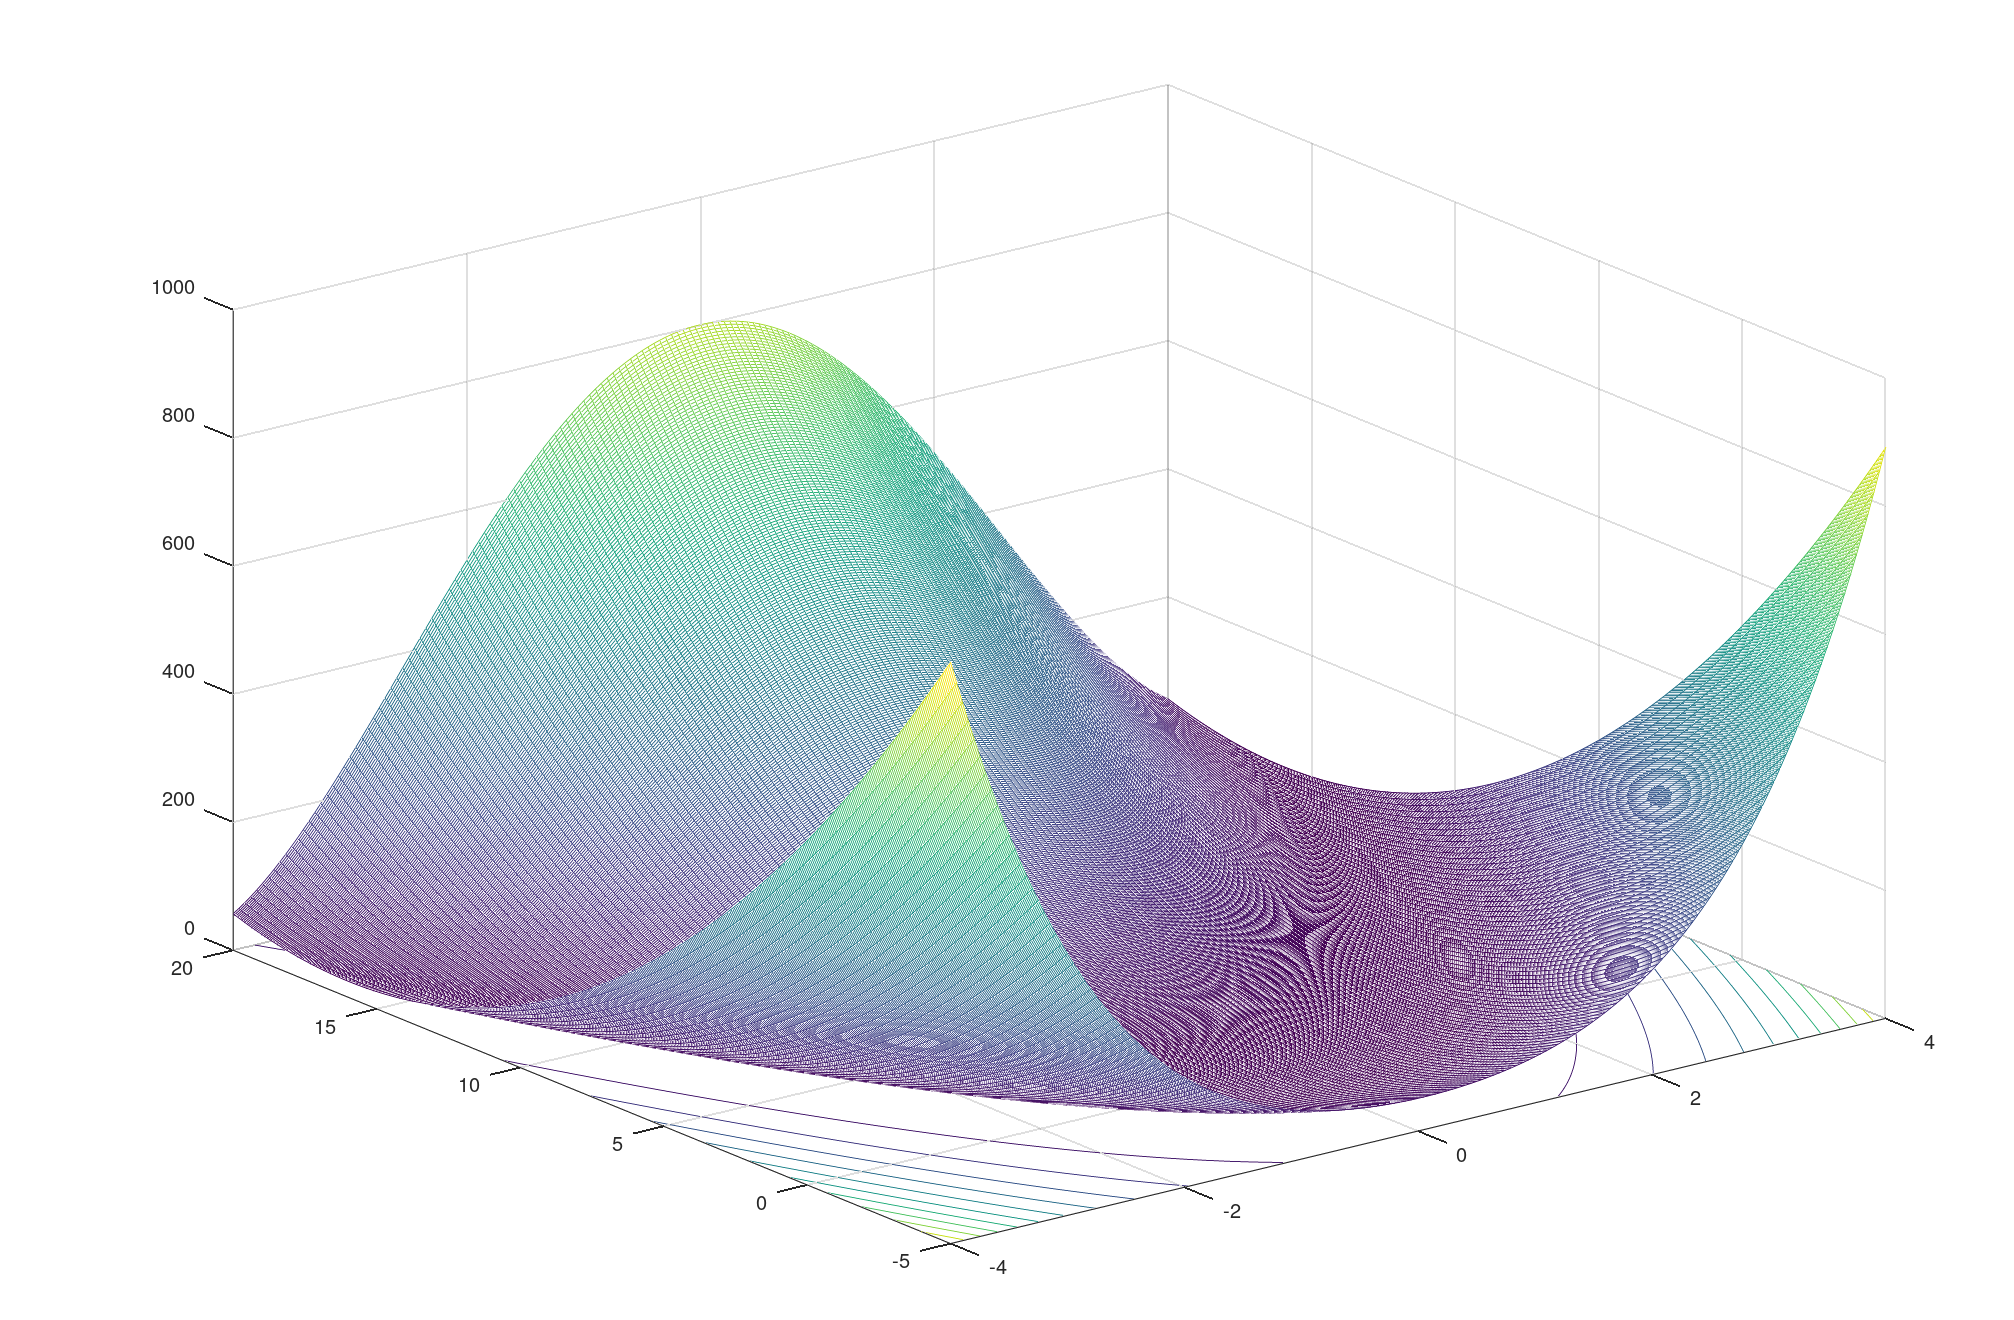
\includegraphics[width=\textwidth]{rosenbrock3D}
        \caption{Visualisation de la fonction de Rosenbrock en 3D}
    \end{subfigure}
    \begin{subfigure}[h]{0.49\textwidth}
        \centering
        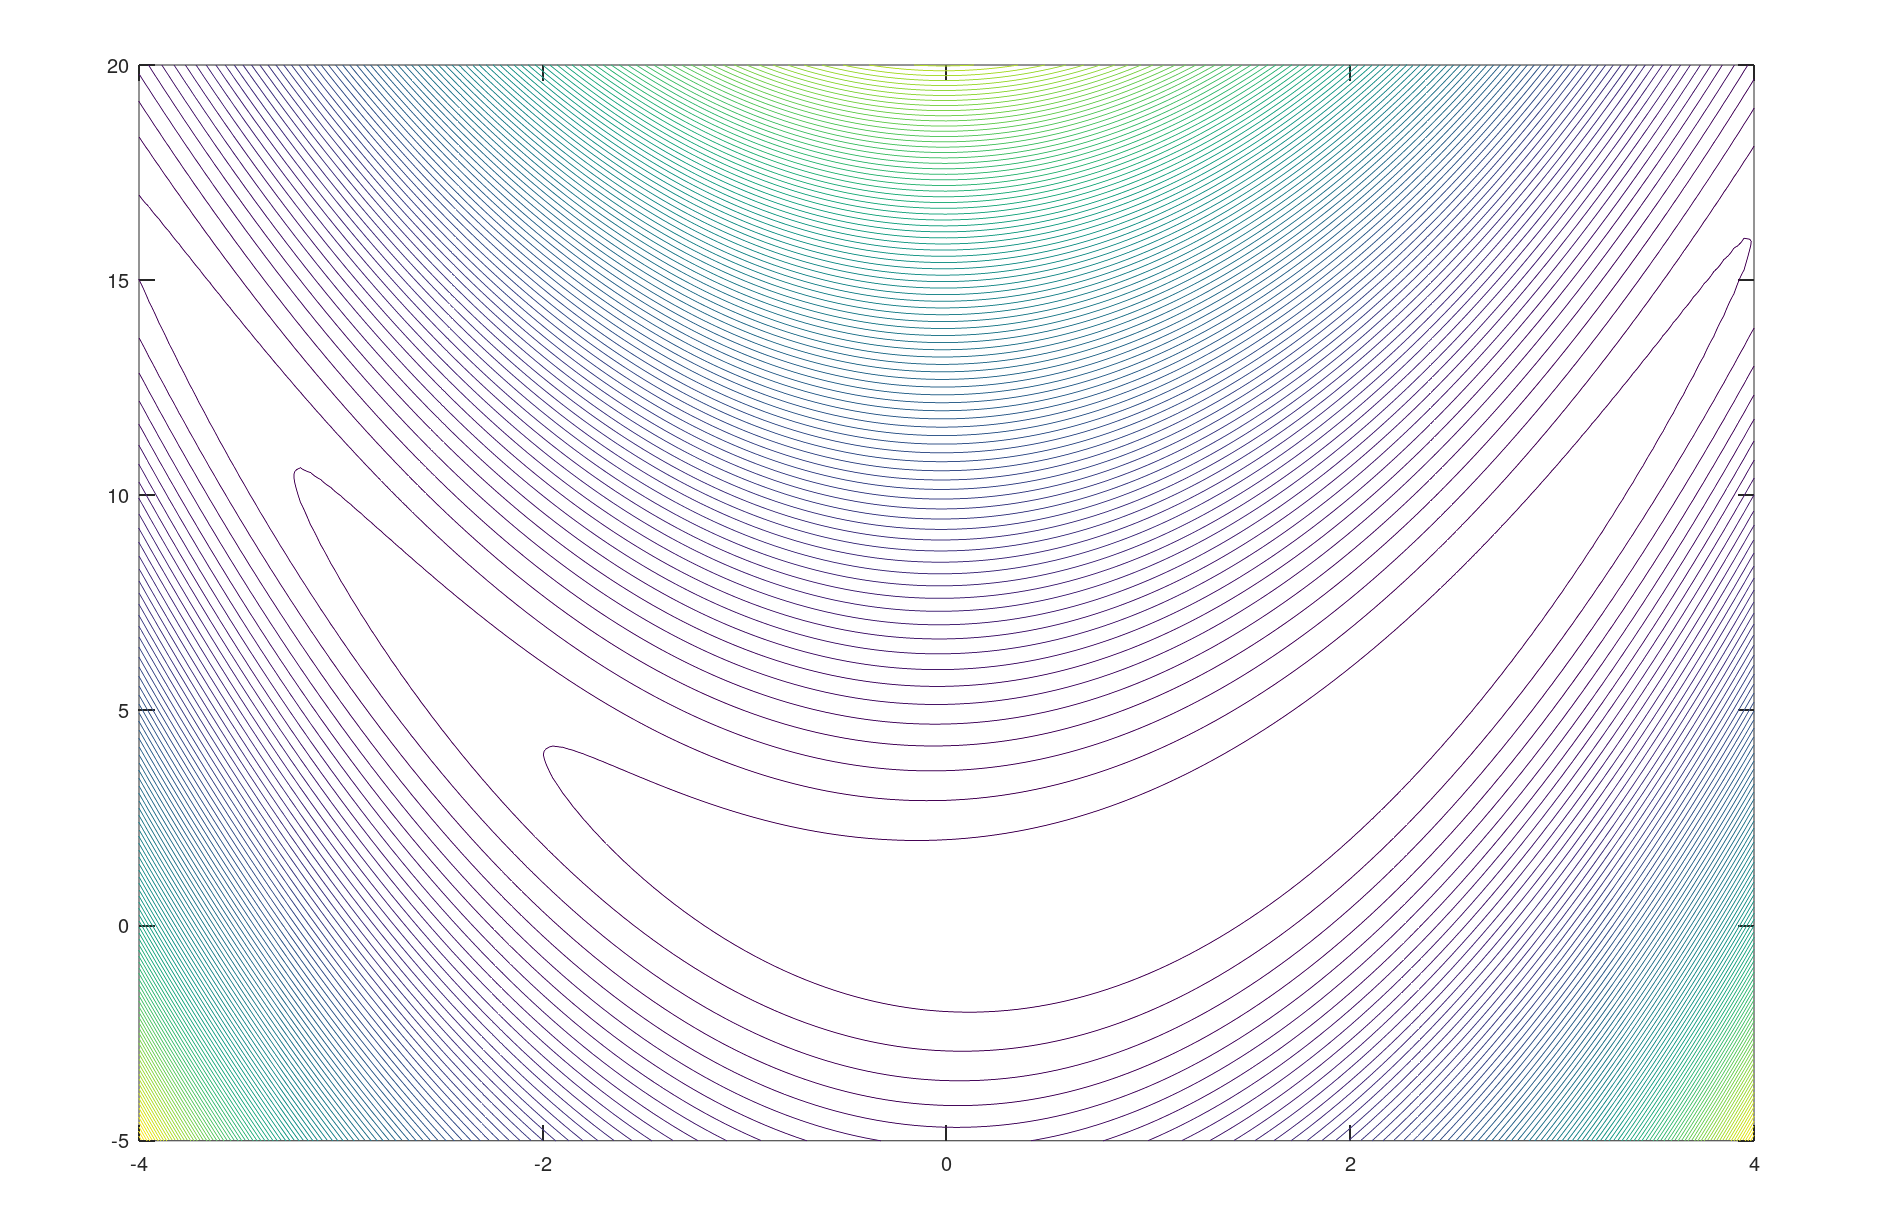
\includegraphics[width=\textwidth]{contourRosenbrock}
        \caption{Visualisation des lignes de niveaux de la fonction}
    \end{subfigure}
\end{figure}

\subsection{Minimisation par descente itérative}

\begin{enumerate}
    \item{
            Pour commencer, on utilise la méthode de descente de plus forte pente avec un pas fixe.
            On obtient alors en 1000 itérations les différents figures : 
            \begin{figure}[H]
                \centering
                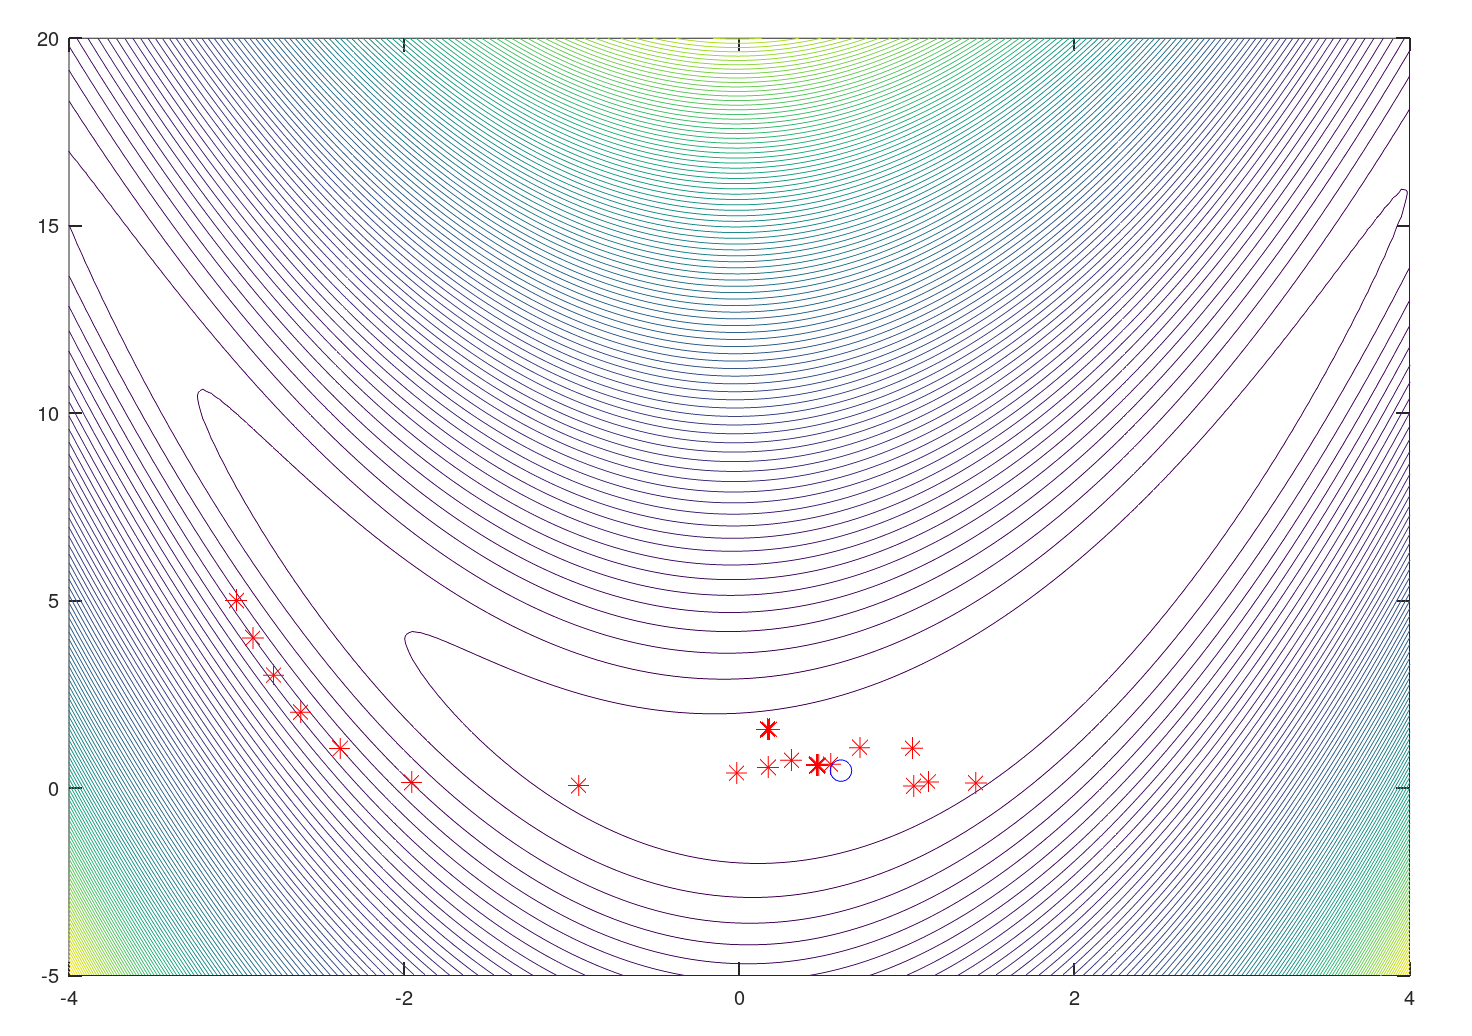
\includegraphics[width=7cm, height=4cm]{pasFixe1}
                \caption{Descente de pas 1}
            \end{figure}

            \begin{figure}[H]
                \centering
                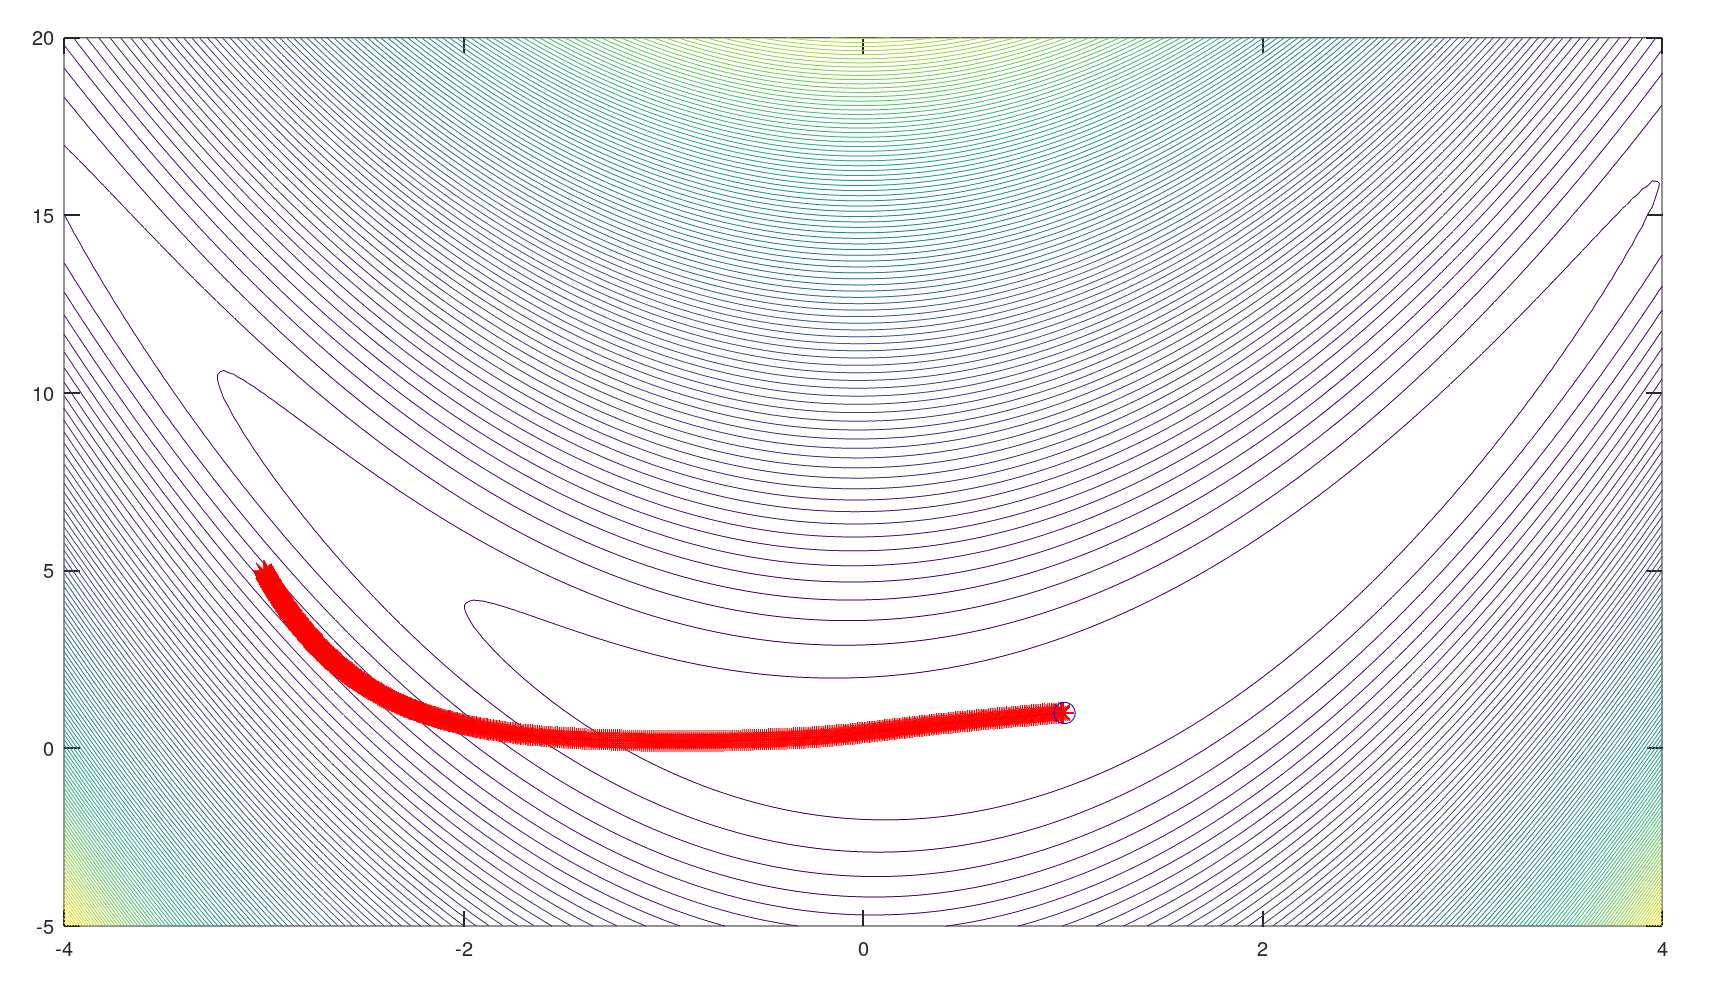
\includegraphics[width=7cm, height=4cm]{pasFixe10moins2}
                \caption{Descente de pas $10^{-2}$}
            \end{figure}

            \begin{figure}[H]
                \centering
                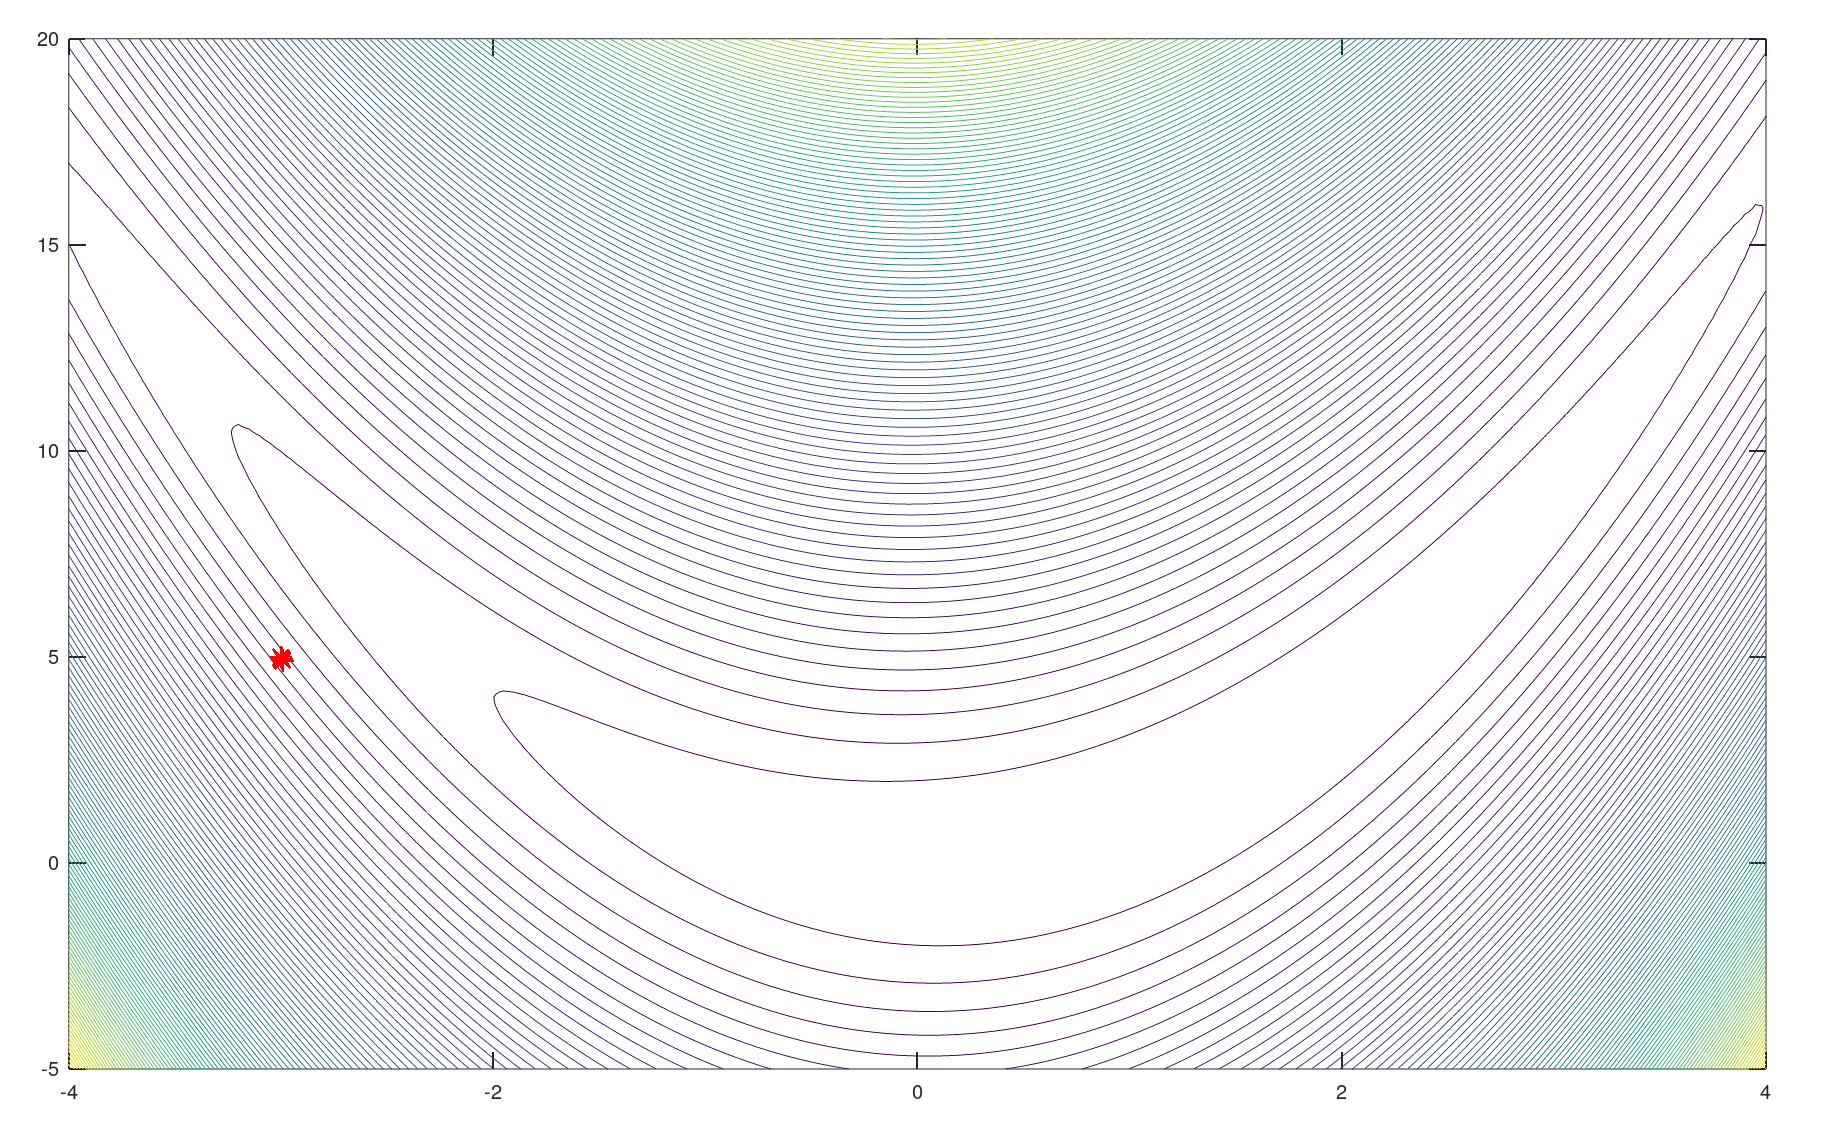
\includegraphics[width=7cm, height=4cm]{pasFixe10moins4}
                \caption{Descente de pas $10^{-4}$}
            \end{figure}

            On remarque que :
            \begin{itemize}
                \item{Avec le pas de $10^{-4}$, les 1000 itérations ne sont pas suffisante pour tendre vers $ x_h$}
                \item{Pour les deux autres valeurs du pas, la méthode converge vers $x_h$ mais avec le pas de 1, la méthode converge bien plus rapidement qu'avec le pas de $10^{-2}$.}
            \end{itemize}
        }

    \item{On ajoute alors une recherche de pas par une technique de rebroussement avec un taux $\beta = 0.75$ pour assurer la condition d'Armijo avec $c=10^{-4}$.

            \begin{figure}[H]
                \centering
                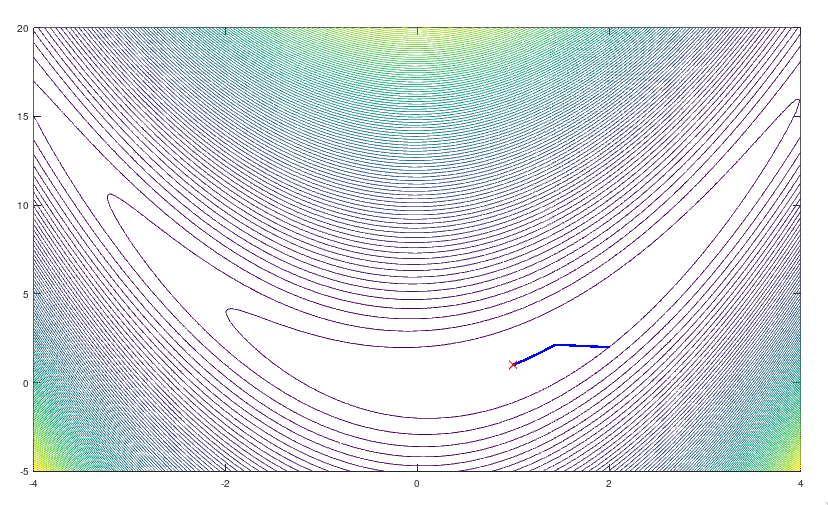
\includegraphics[width=7cm, height=4cm]{pasVar}
                \caption{technique de rebroussement}
            \end{figure}

            On observe alors que le pas varie effectivement au cours des itérations, de sorte à assurer la
            condition d'Armijo, ce qui garantit une décroissance suffisante et permet donc de ne pas avoir à se
            soucier des problèmes vus plus haut (pas trop faible ou trop élevé). Cependant, cette méthode est
            plus stable mais nécessite plus de calculs que pour la méthode du pas fixe, elle est par exemple 
            bien plus lente que la méthode de pas fixe avec un pas de 1 pour cet exemple précis.
        }

        \setcounter{enumi}{3}
    \item{
            Pour la valeur : $x_0 = (4, 4)$, on obtient les tracés suivants :

            \begin{figure}[H]
                \centering
                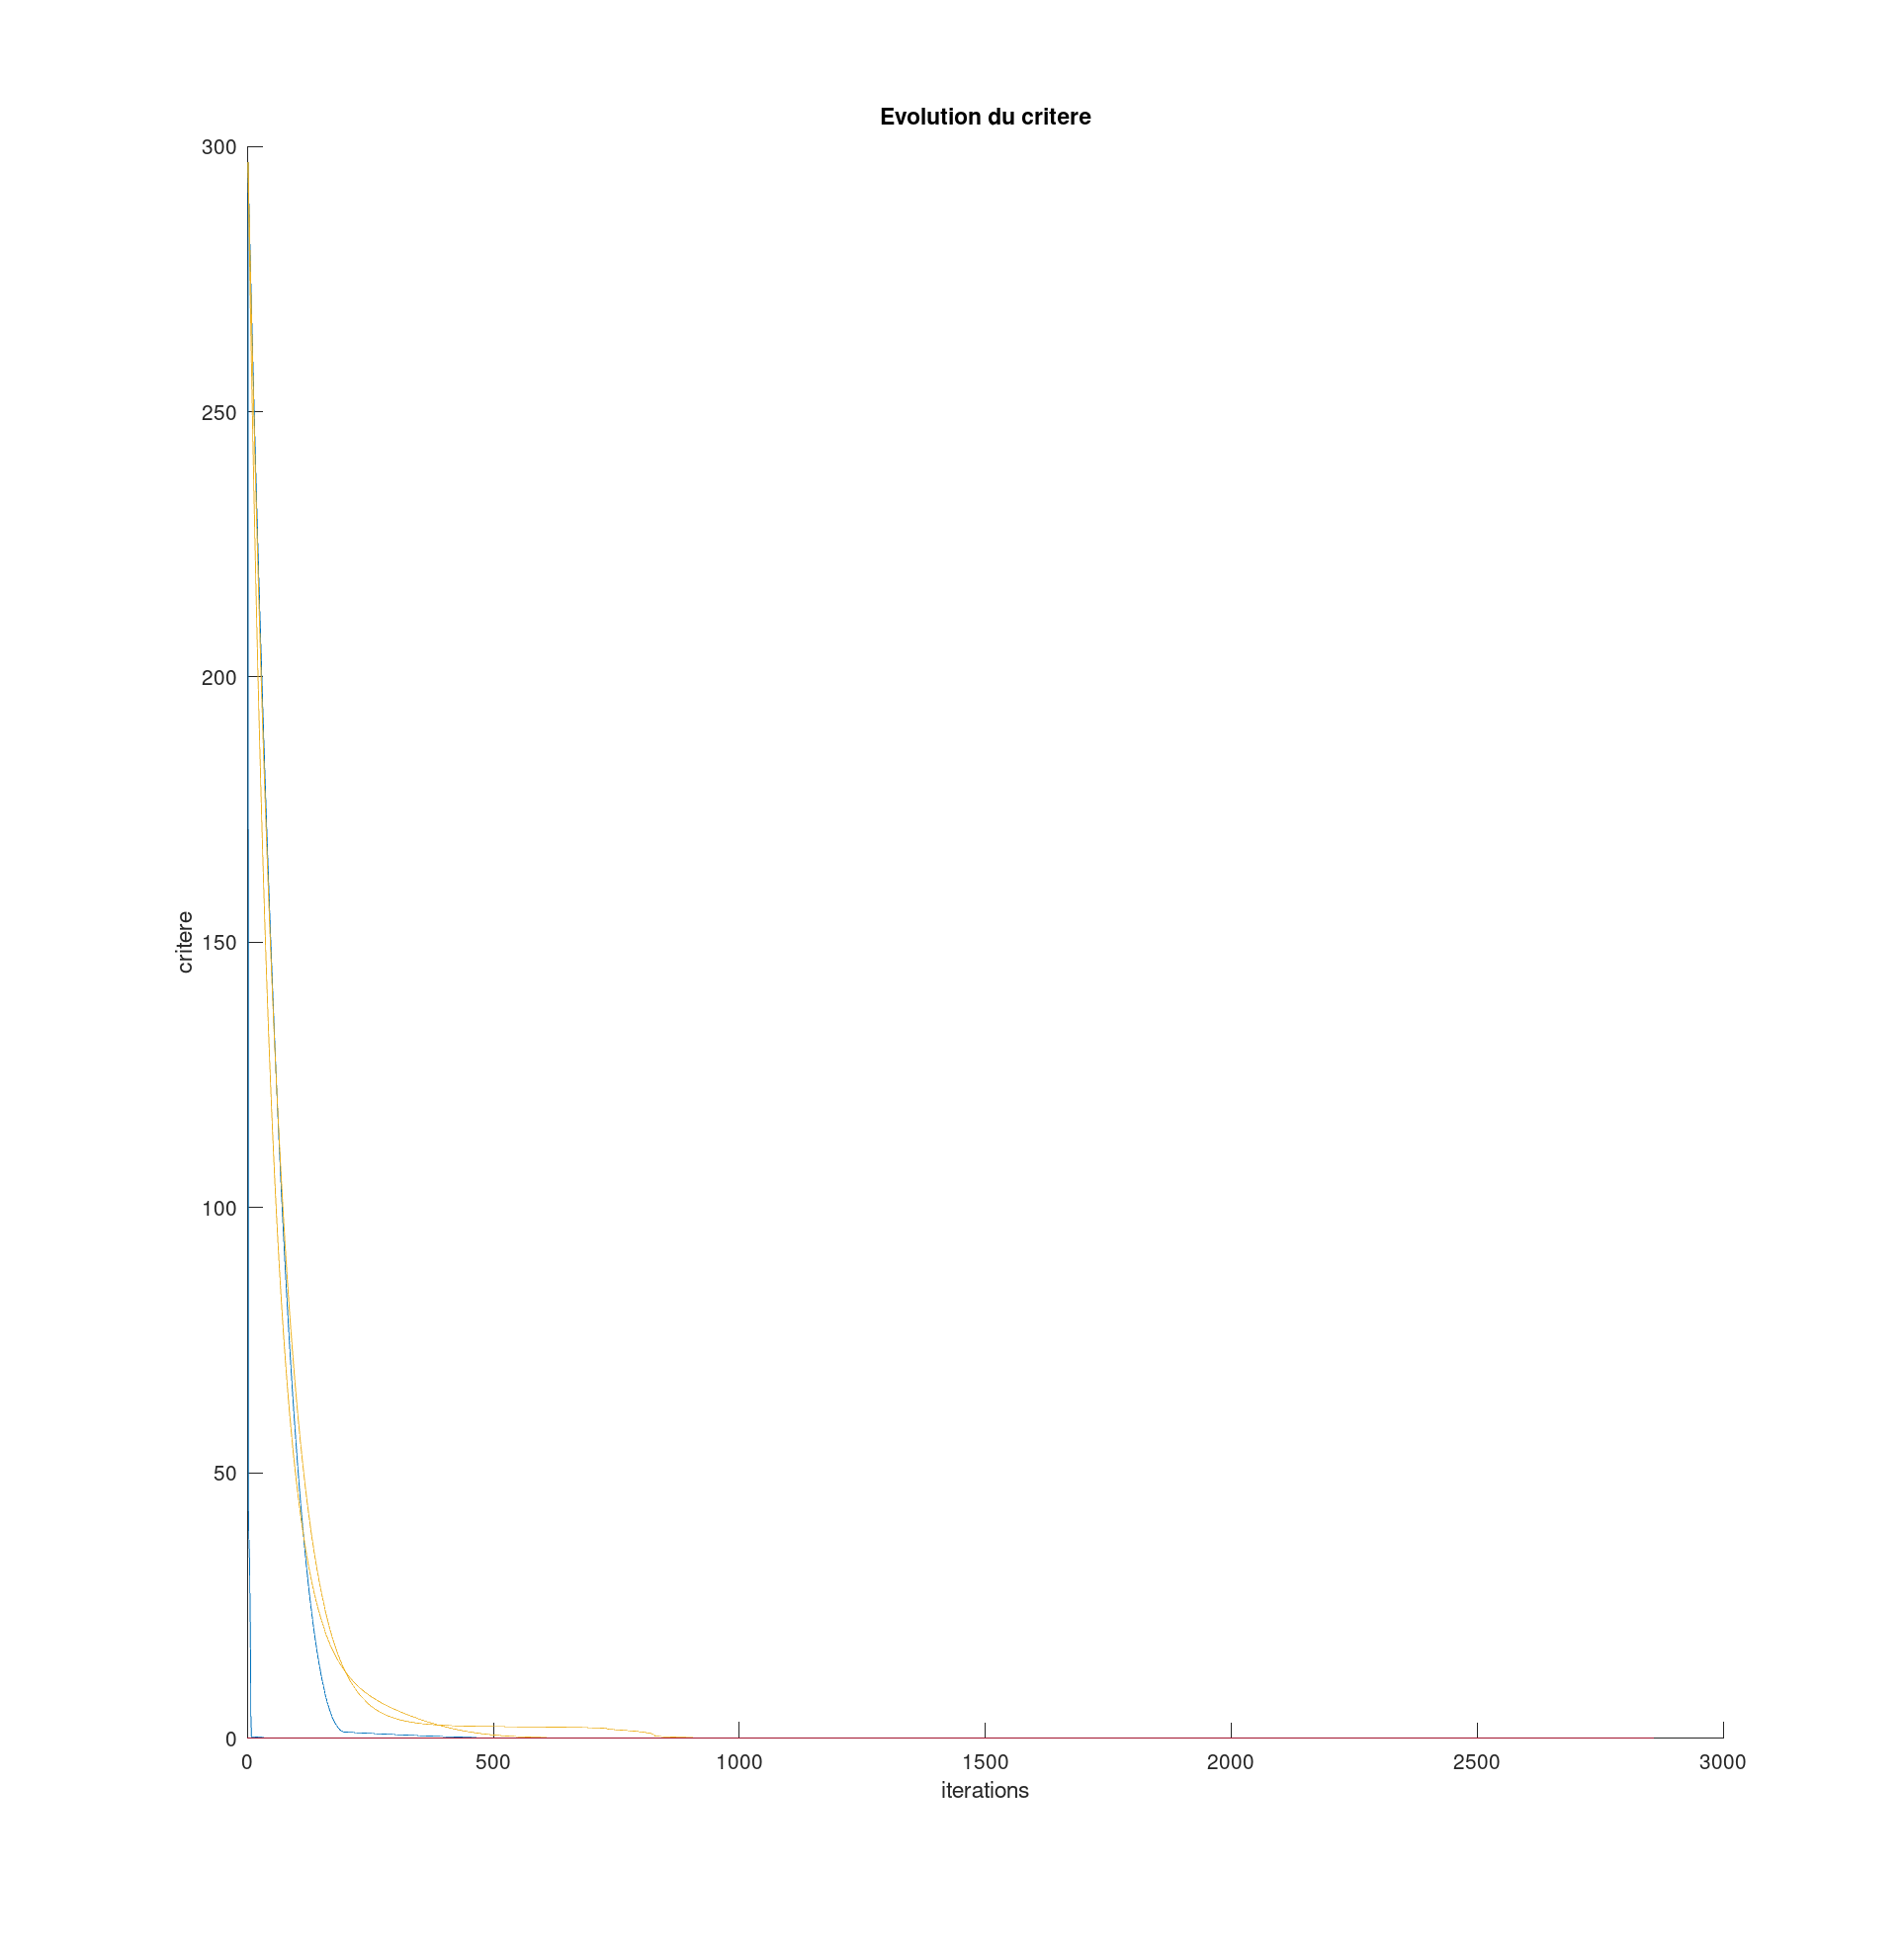
\includegraphics[width=0.5\textwidth]{critere}
                \caption{Évolution du critère}
            \end{figure}

            \begin{figure}[H]
                \centering
                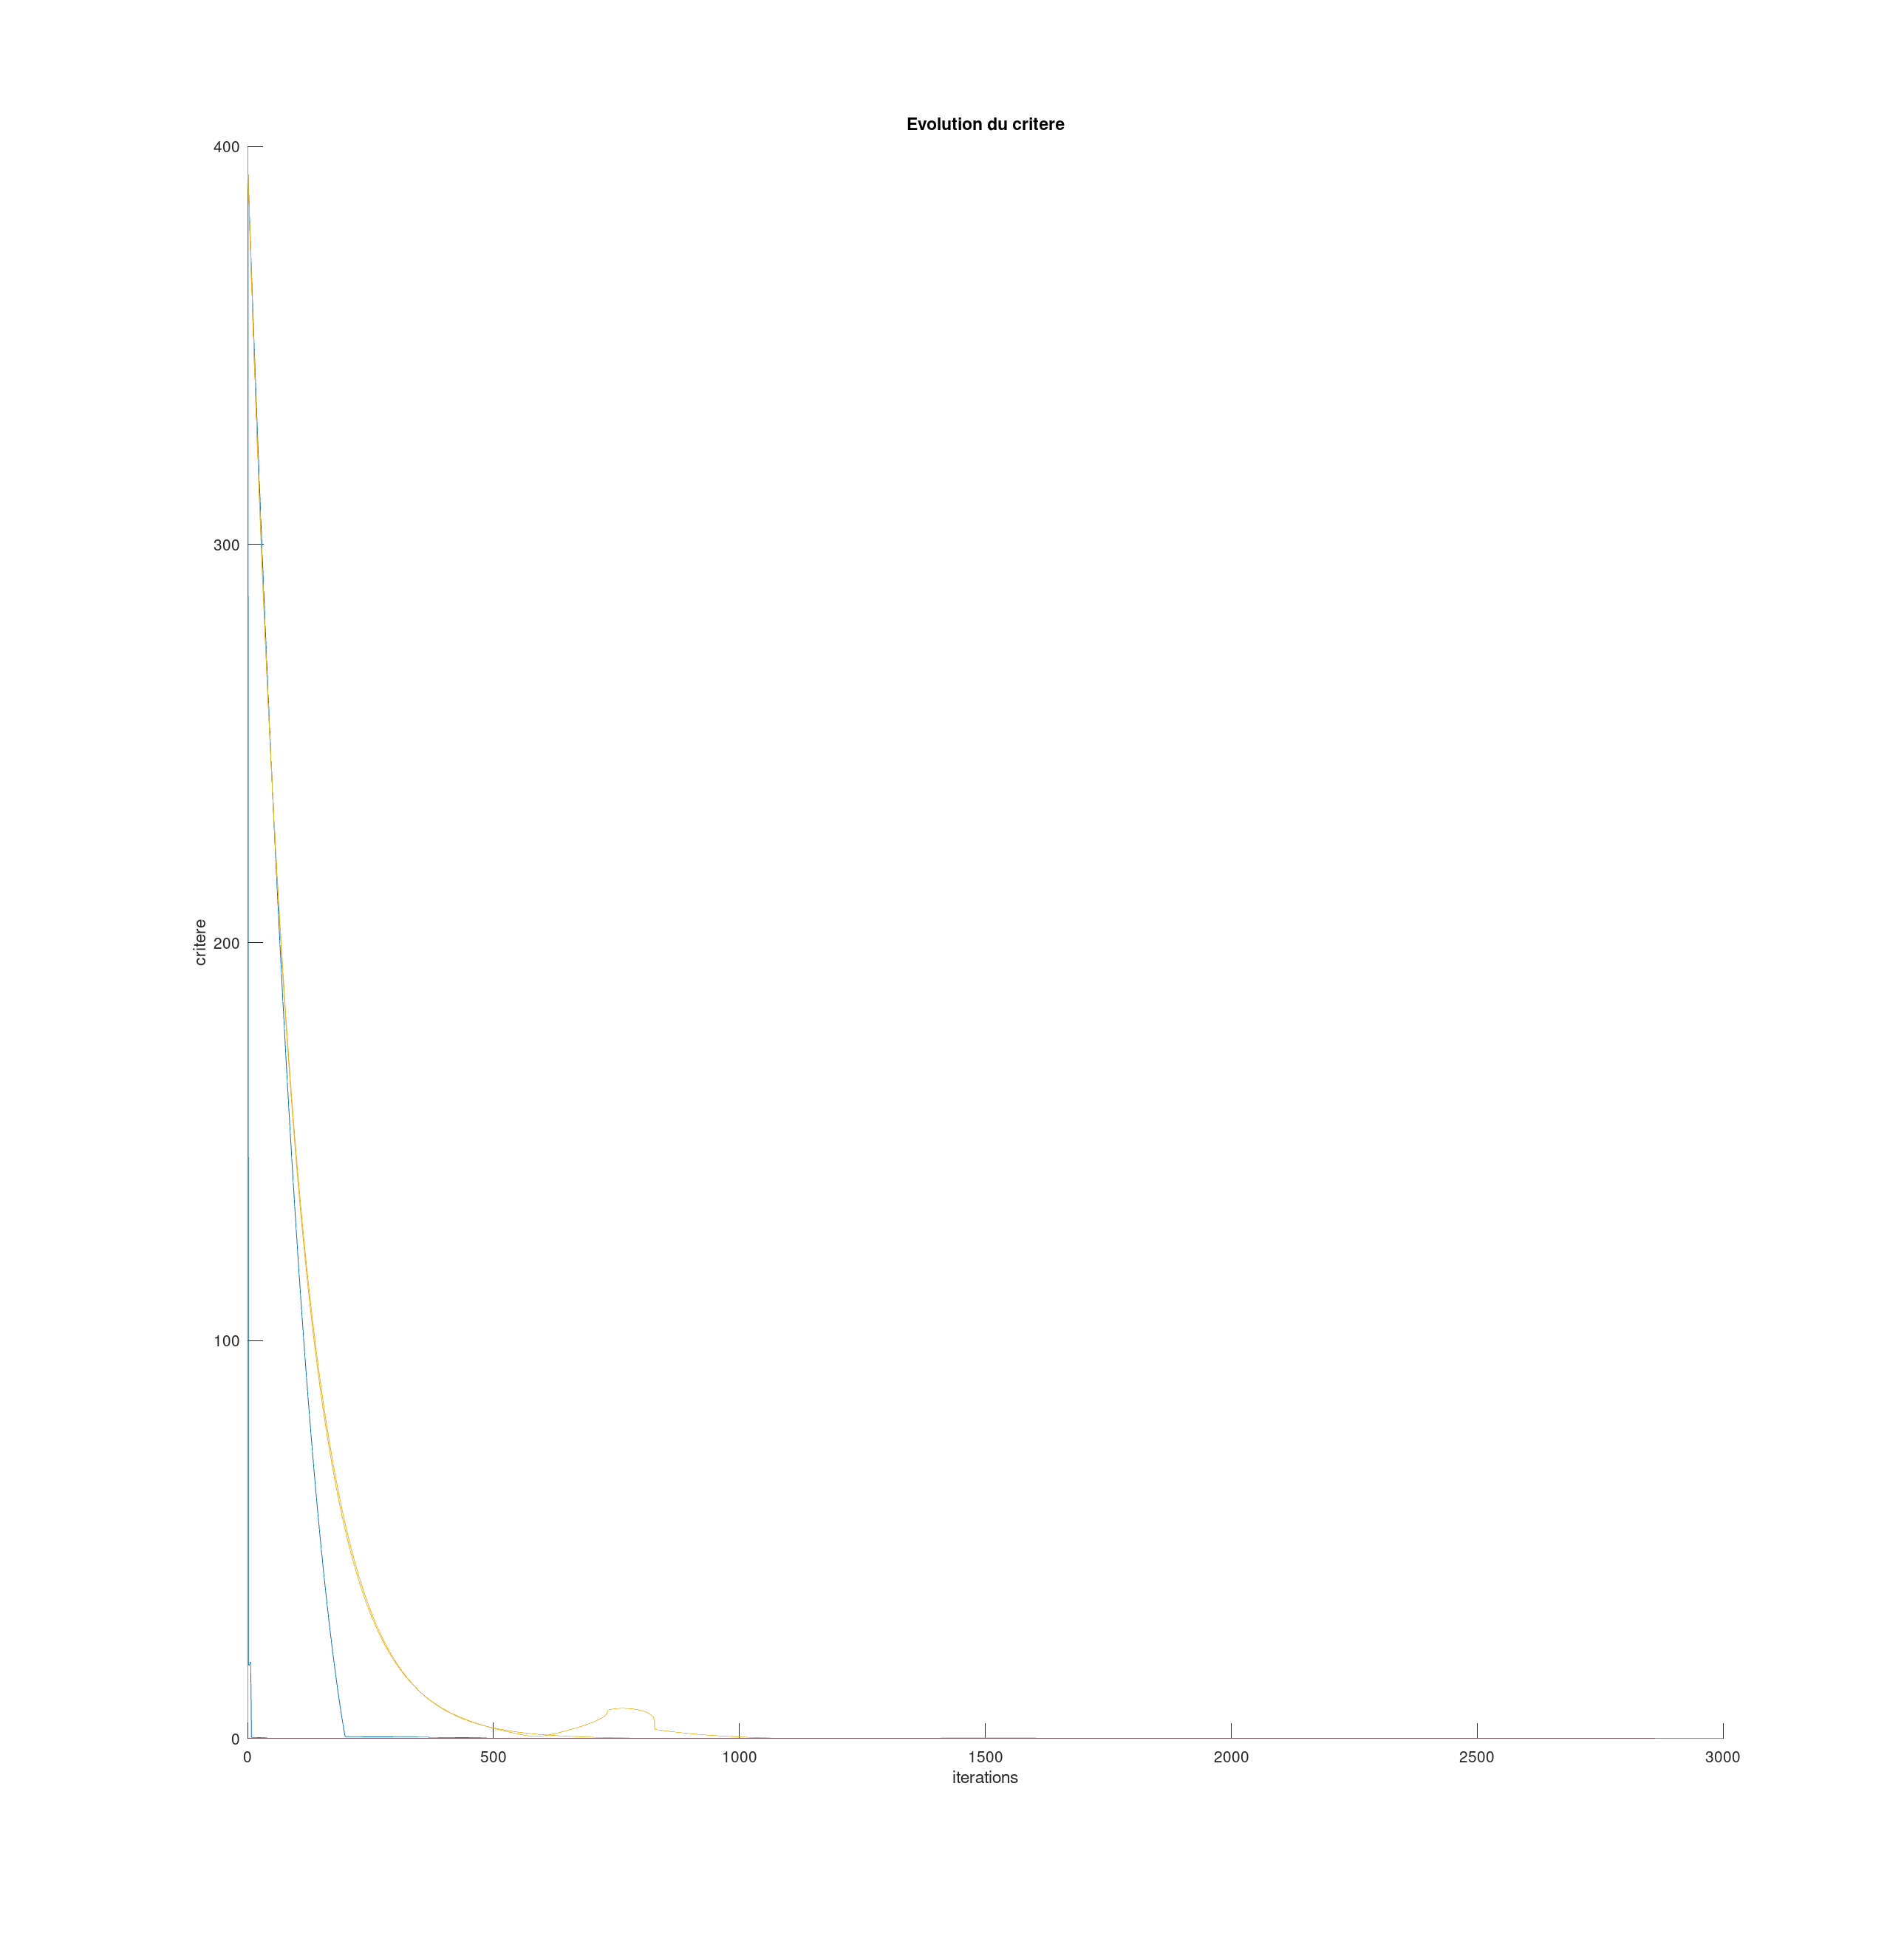
\includegraphics[width=0.5\textwidth]{gradient}
                \caption{Évolution de la norme du gradient}
            \end{figure}

            Pour la valeur : $x_0 = (5, 10)$ et avec un pas variable, on obtient les tracés suivants :

            \begin{figure}[H]
                \centering
                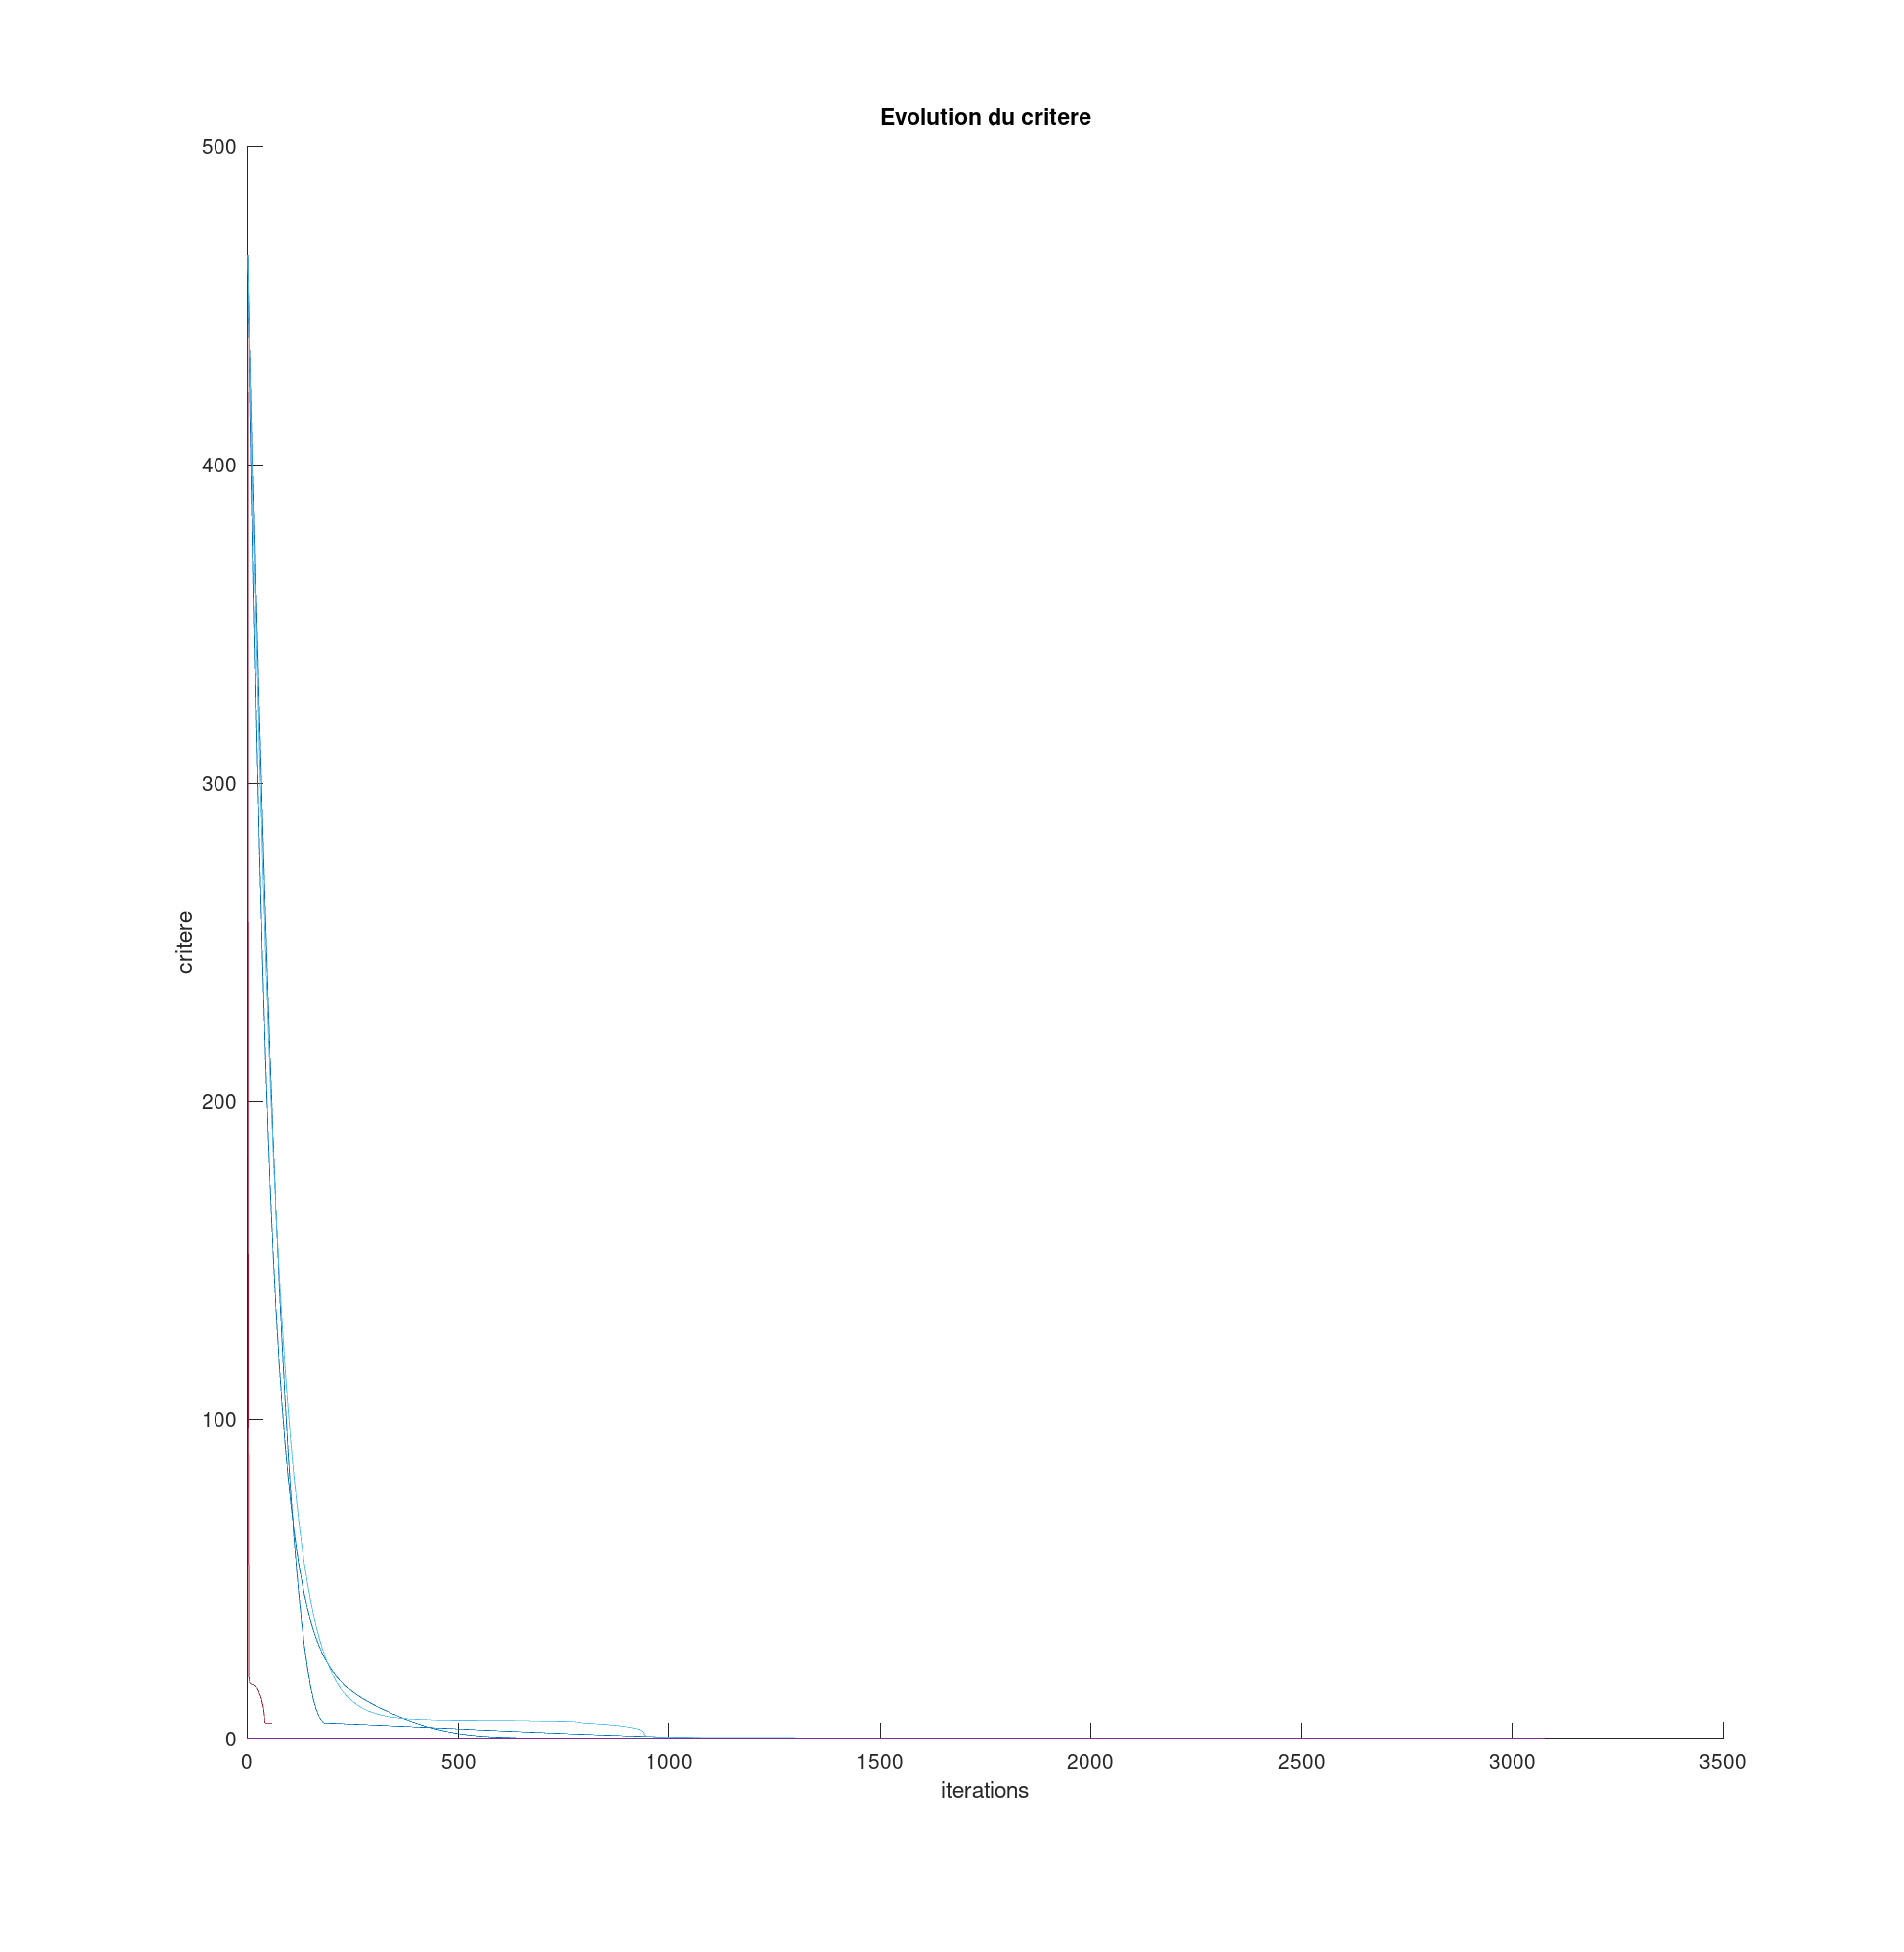
\includegraphics[width=0.5\textwidth]{critere2}
                \caption{Évolution du critère}
            \end{figure}

            \begin{figure}[H]
                \centering
                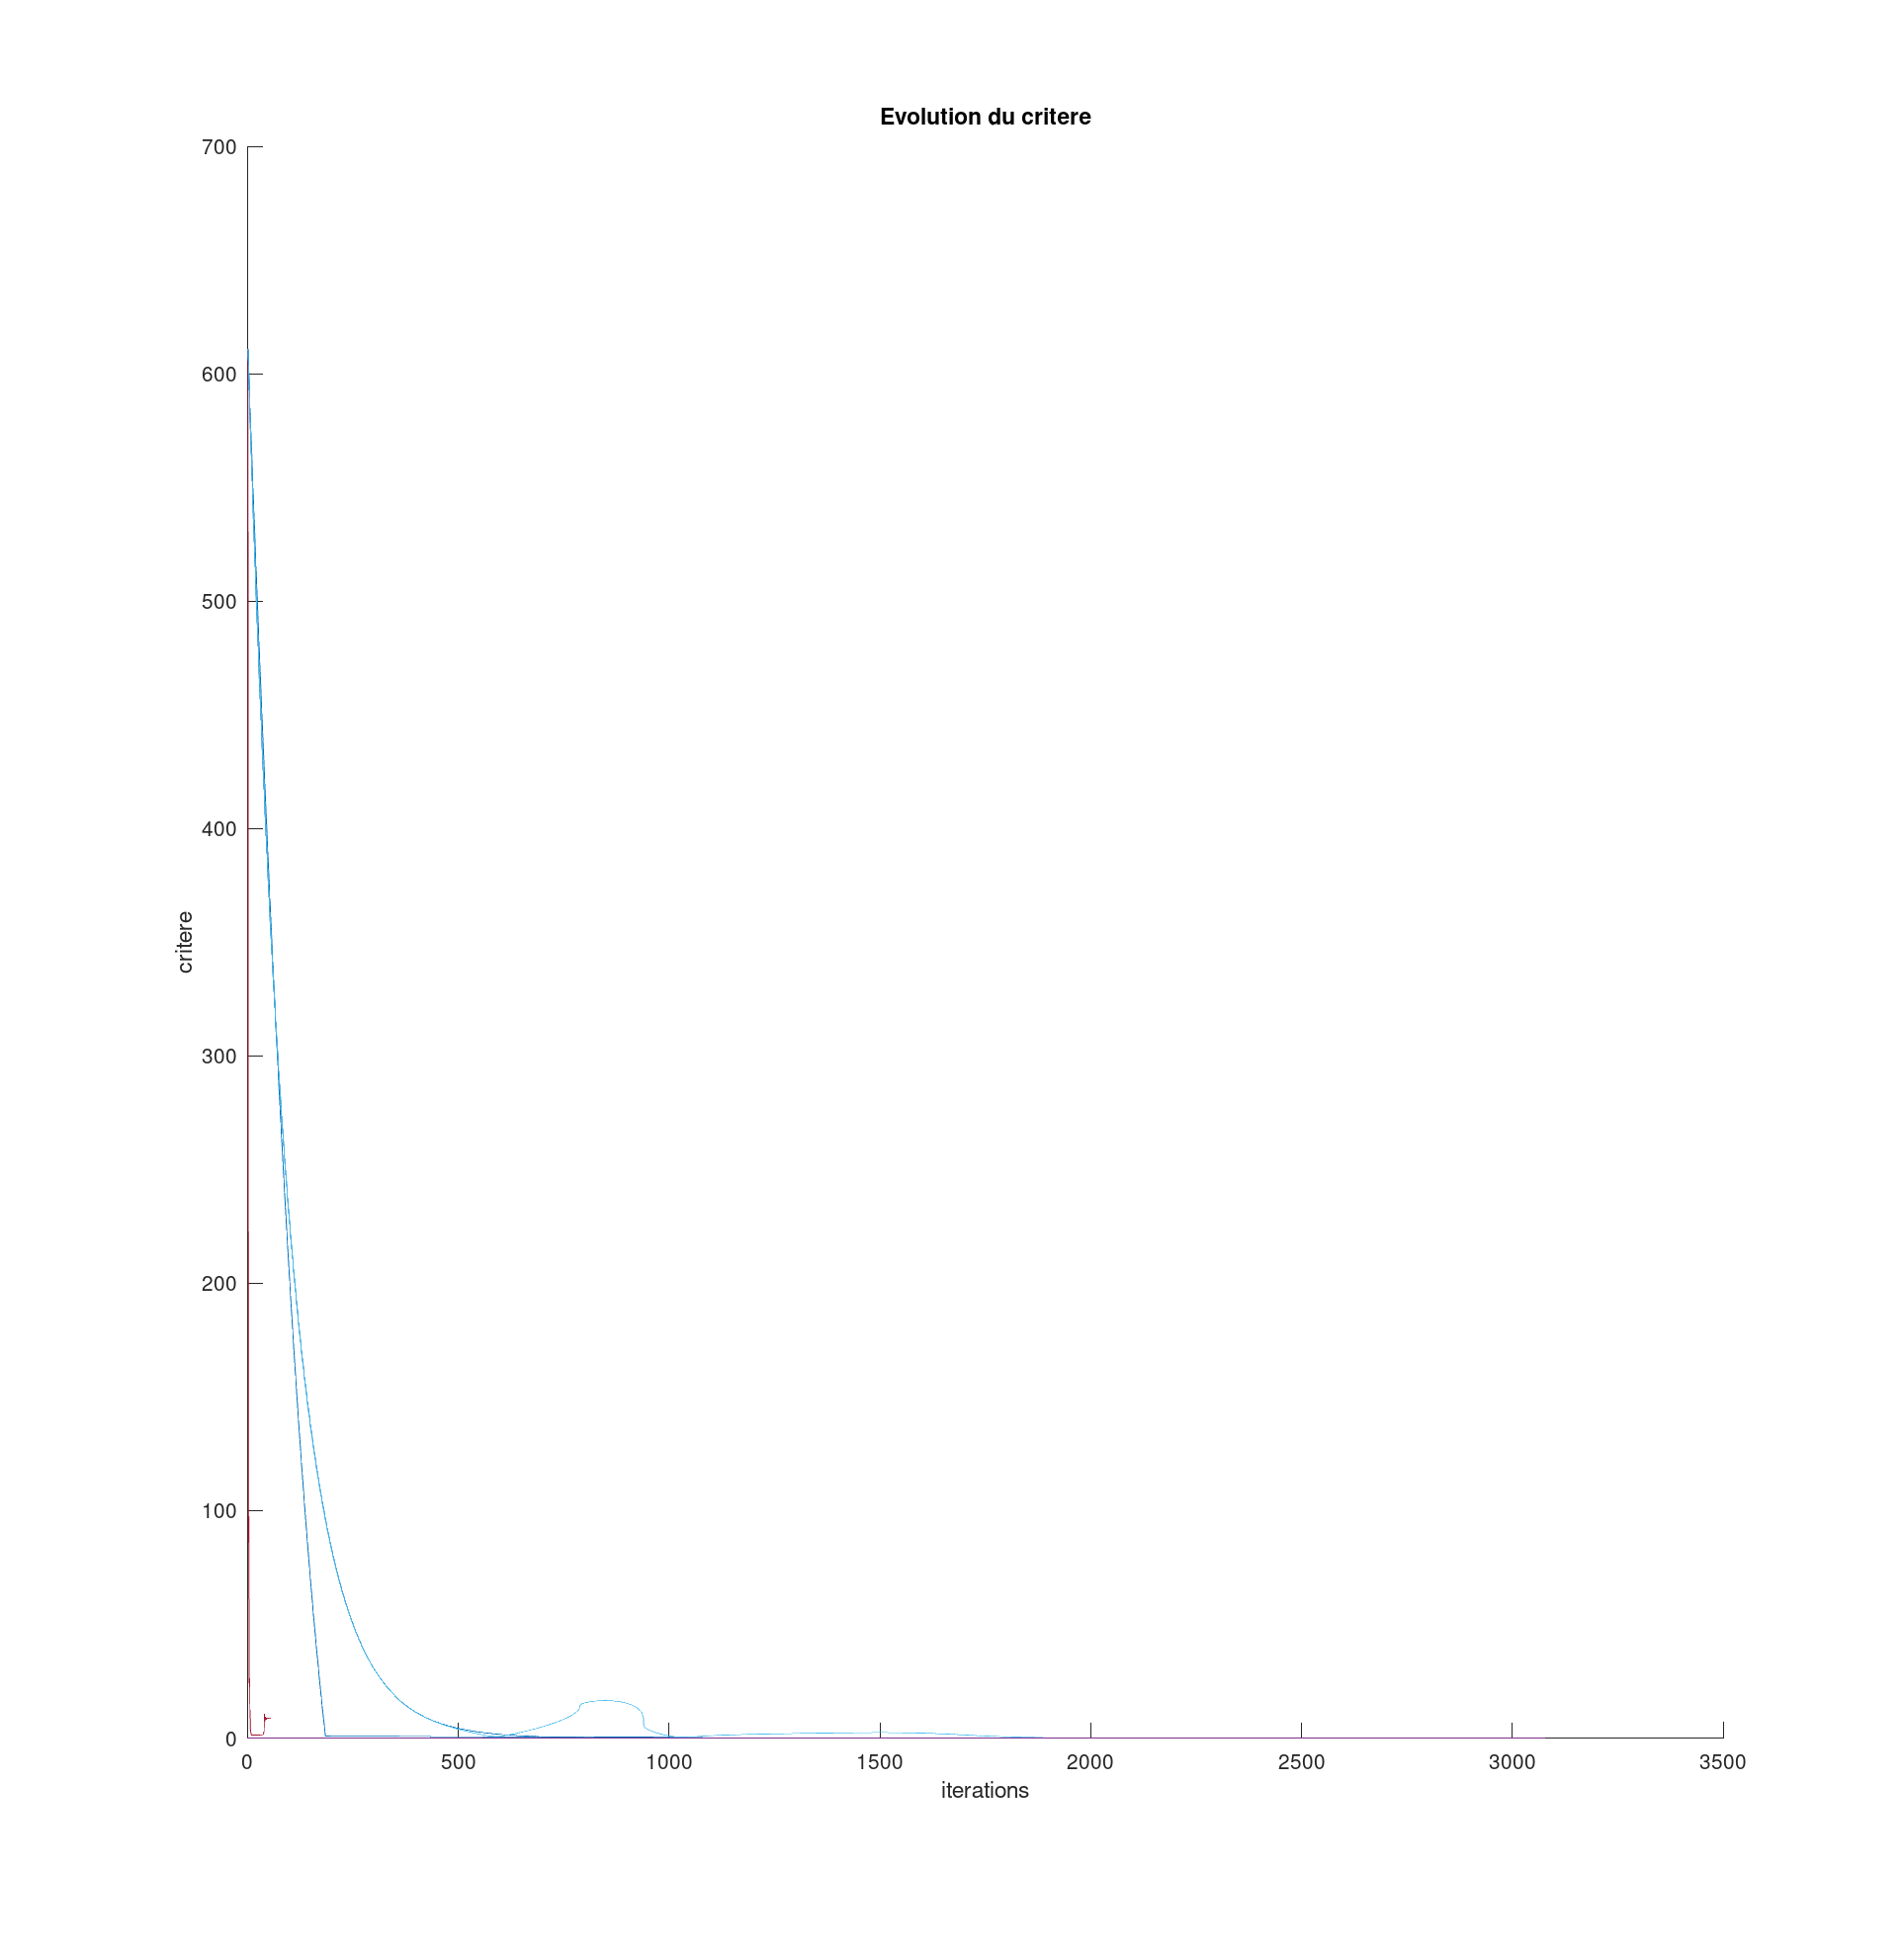
\includegraphics[width=0.5\textwidth]{gradient2}
                \caption{Évolution de la norme du gradient}
            \end{figure}

            Nous avons cependant plusieurs problèmes d'affichage de ces graphiques sous Octave
            (nous n'arrivons par exemple pas à afficher la légende ou à interagir avec les tracés).
            On observe tout de même que pour ces 4 tracés le critère et le gradient s'annulent
            rapidement pour chaque méthode, il faudrait choisir des valeurs de tolérance plus
            adaptées pour gagner en temps d'exécution, quitte à être légèrement moins précis.
            Pour comparer les performances de chaque méthode représentons le nombre d'itérations
            et le temps d'exécution dans un tableau :

            Pour $x_0 = (4,4)$ :

            \begin{table}[H]
                \begin{tabularx}{\textwidth}{ |l|X|X| }
                    \hline
                    Méthode & Nombre d'itérations & Temps (s) \\
                    \hline
                    Descente de plus forte pente & 911 & 0.51 \\
                    \hline
                    Gradient conjugué & 451  & 0.18 \\
                    \hline
                    Newton & 1989 & 0.37 \\
                    \hline
                    BFGS & 2862 & 0.75 \\
                    \hline
                \end{tabularx}
            \end{table}

            Pour $x_0 = (5,10)$ :

            \begin{table}[H]
                \begin{tabularx}{\textwidth}{ |l|X|X| }
                    \hline
                    Méthode & Nombre d'itérations & Temps (s) \\
                    \hline
                    Descente de plus forte pente & 1526 & 0.70 \\
                    \hline
                    Gradient conjugué & x & x \\
                    \hline
                    Newton & 2043 & 0.64 \\
                    \hline
                    BFGS & 3000 & 1.30 \\
                    \hline
                \end{tabularx}
            \end{table}

            On remarque alors que :

            \begin{itemize}
                \item{Pour la première valeur de $x_0$, la méthode du gradient conjuguée est la
                    plus performante que ce ce soit en temps de calcul ou en nombre d'itérations}
                \item{Mais la méthode du gradient conjuguée ne converge pas vers $x_h$ pour une
                    position initiale plus éloignée.}
                \item{Les méthodes de Newton et BFGS sont celles nécessitant le plus d'itérations}
                \item{La méthode de Newton est cependant plus rapide que celle du gradient de plus
                    forte pente}
            \end{itemize}

        }

        \setcounter{enumi}{5}
    \item{
            Pour $x_0 = (4,4)$ :

            \begin{table}[H]
                \begin{tabularx}{\textwidth}{ |l|X|X| }
                    \hline
                    Méthode & Nombre d'itérations & Temps (s) \\
                    \hline
                    Gauss-Newton & 1603 & 0.31 \\
                    \hline
                    levenberg-marquardt & 1594 & 0.33 \\
                    \hline
                \end{tabularx}
            \end{table}

            Pour $x_0 = (5,10)$ :

            \begin{table}[H]
                \begin{tabularx}{\textwidth}{ |l|X|X| }
                    \hline
                    Méthode & Nombre d'itérations & Temps (s) \\
                    \hline
                    Gauss-Newton & 1622 & 0.32 \\
                    \hline
                    levenberg-marquardt & 1607 & 0.35 \\
                    \hline
                \end{tabularx}
            \end{table}

            On remarque alors que :

            \begin{itemize}
                \item{Les deux méthodes convergent bien vers $x_h$ pour les deux valeurs de $x_0$.}
                \item{Les performances de ces deux méthodes sont très similaires pour les
                        deux valeurs de $x_0$, ce qui n'est pas le cas des autres méthodes et
                    qui représente un avantage important.}
                \item{Ce sont les méthodes les plus rapides pour la deuxième valeur de $x_0$ et
                    la deuxième plus rapide pour la première valeur de $x_0$.}
                \item{La méthode de levenberg-marquardt nécessite le choix d'une valeur pour
                        un paramètre. Dans ce cas ci, nous obtenons des résultats satisfaisant
                        uniquement pour des valeurs très faibles de $\lambda$, la méthode est 
                    alors quasiment équivalente à celle de Gauss-Newton.}
            \end{itemize}
        }

\end{enumerate}

\newpage
\section{Ajustement d'une courbe non-linéaire}

\newpage
\section{Débruitage d’un signal par minimisation d ’un critère composite}

\newpage
\section{Inversion numérique d’une transformée de Laplace par optimisation sous contraintes}

\newpage

\begin{appendices}

    \section{Minimisation de la fonction de Rosenbrock}

    \subsection{\texttt{rosenbrock.m}}

    \lstinputlisting[language=Matlab]{../rosenbrock.m}

    \subsection{\texttt{optimdescent.m}}

    \lstinputlisting[language=Matlab]{../optimdescent.m}

    \subsection{\texttt{main_tpcsopt_optim1.m}}

    \lstinputlisting[language=Matlab]{../main_tpcsopt_optim1.m}

    \subsection{\texttt{visualisation.m}}

    \lstinputlisting[language=Matlab]{../visualisation.m}

    \subsection{\texttt{comparaison.m}}

    \lstinputlisting[language=Matlab]{../comparaison.m}

\end{appendices}

\end{document}
